\documentclass[10pt,a4paper,twoside]{article} 
\usepackage[latin1]{inputenc}
\usepackage[english]{babel}
\usepackage{amsmath}
\usepackage{amsfonts}
\usepackage{amssymb}
\usepackage{makeidx}
\usepackage{graphicx}
\usepackage{hyperref}
\usepackage[left=2cm,right=2cm,top=2cm,bottom=2cm]{geometry}
\usepackage{float}
\usepackage{multirow}
\usepackage{verbatim} %for å kommentere ut ting
\usepackage[nottoc,numbib]{tocbibind}
\usepackage[parfill]{parskip} %for avsnitt
\usepackage{listings}
    \lstset{
            language=Matlab,                                % choose the language of the code
    %       basicstyle=10pt,                                % the size of the fonts that are used for the code
            numbers=left,                                   % where to put the line-numbers
            numberstyle=\footnotesize,                      % the size of the fonts that are used for the line-numbers
            stepnumber=1,                                           % the step between two line-numbers. If it's 1 each line will be numbered
            numbersep=5pt,                                  % how far the line-numbers are from the code
    %       backgroundcolor=\color{white},          % choose the background color. You must add \usepackage{color}
            showspaces=false,                               % show spaces adding particular underscores
            showstringspaces=false,                         % underline spaces within strings
            showtabs=false,                                         % show tabs within strings adding particular underscores
    %       frame=single,                                           % adds a frame around the code
    %       tabsize=2,                                              % sets default tabsize to 2 spaces
    %       captionpos=b,                                           % sets the caption-position to bottom
            breaklines=true,                                        % sets automatic line breaking
            breakatwhitespace=false,                        % sets if automatic breaks should only happen at whitespace
            escapeinside={\%*}{*)}                          % if you want to add a comment within your code
    }

\raggedbottom

\usepackage{makeidx}
\makeindex
%symbolliste slutt

\author{Anders Dall'Osso Teigset}
\title{MEDIUM VOLTAGE LOAD BREAK SWITCH WITH AIR AS INTERRUPTING MEDIUM}
\date{December, 2013}


\begin{document}
    \begin{titlepage}
    \begin{center}
    \ \\
    \ \\
    \ \\
    \ \\
    \ \\
    \ \\
    Anders Dall'Osso Teigset \\
    \ \\
    \ \\
    \ \\
    \ \\{\large \bfseries
    MEDIUM VOLTAGE LOAD BREAK SWITCH WITH AIR AS INTERRUPTING MEDIUM\\
    }
    \ \\
    \ \\
    \ \\
    \ \\
    \ \\
    {\large
    Specialisation project\\
    }
    \ \\
    {December, 2013 \\}
    \ \\
    \ \\
    \ \\
    \ \\
    \ \\
    \ \\
    \ \\
    \ \\
    \ \\
    \ \\
    \ \\
    \ \\
    \ \\
    \ \\
    \ \\
    \ \\
    \ \\
    \ \\
    \ \\
    \ \\
    \ \\
    \ \\
    \ \\
    \ \\
    \ \\
    \ \\
    \ \\
    \ \\
    \ \\
   	{\large
   Norwegian University of Science and Technology\\
   Department of Electric Power Engineering\\
    }
   	\ \\
    \ \\
    \ \\
    \ \\
    \end{center}
    \end{titlepage}

%\maketitle
%SummaryNyttige pdf-filer/SF6conduct.pdf
\thispagestyle{empty}
\cleardoublepage
\section*{Acknowledgements}
\setcounter{page}{1}
\pagenumbering{roman}

\cleardoublepage
\section*{Summary}

\cleardoublepage
\setcounter{page}{1}
\pagenumbering{arabic}
\tableofcontents
\cleardoublepage

\section{Introduction}

\cleardoublepage

\section{Theory}
\subsection{Typical switchgear design and interruption sequence} \label{sec:genDes}
Most of the information in section \ref{sec:genDes} is collected from \textit{"Current Interruption in Power Grids"} by Magne Runde \cite{bib:HVEbreak} \newline

\subsubsection{Switchgear design and operation} \label{sec:InterruptCurrent}
Switchgear can be divided into four main categories:
\begin{itemize}
\item Disconnector Switch
\item Load Break Switch
\item Circuit Breaker
\item Earthing Switch
\end{itemize}

This report will focus on the load break switch (LBS) design. An LBS is designed to be able to interrupt currents with a magnitude equal to or less than the rated maximum continuous current in a transmission system. An LBS should fulfil the following demands in order to meet the requirements of the application area:

\begin{itemize}
\item When closed:
	\begin{itemize}
		\item Act as a good conductor.
		\item Be capable of interrupting any load that may arise, without generating too high over-voltages. 
	\end{itemize}
\item When open:
	\begin{itemize}
		\item Act as a good insulator.
		\item Be able to close without welding the contacts together, even under short-circuit conditions.
	\end{itemize}
\end{itemize}

A typical opening sequence for a switch is as follows: First, a control signal enters the switch and activates the driving mechanisms. In most cases, this is a compressed spring or a hydraulic system. The contacts begin to open, and a gap forms between them. At the same time, an electrical arc ignites between the contacts, burning in the gap. The gap is filled with some kind of interrupting medium which is usually a gas. When an altering current crosses zero, this is referred to as the current zero (CZ). For an alternating current with a frequency of 50 Hz, CZ will occur 100 times per second. Direct current interruptions will not be explained in this report.

%bilde som viser driving mechanisms compressed spring contacts?

At the CZ, the arc will extinguish for at least a moment, because the current is zero, and a voltage will build up between the contacts. This voltage is called the recovery voltage, and is defined in equation \eqref{eq:U_rec}, where $u_{supply}$ is the voltage on the supply side and $u_{load}$ is the voltage on the load side of the open switch. Depending on the recovery voltage two possible scenarios can occur: a re-ignition or a successful quenching of the arc. This is dependent on the steepness and the amplitude of the recovery voltage. There are two different kinds of re-ignition: thermal and dielectric. Thermal re-ignition takes place right after CZ, up to a few microseconds, and is mainly dependent on the steepness of the recovery voltage. As the recovery voltage rises and if a thermal re-ignition is avoided, a dielectric re-ignition may occur. This kind of re-ignition is largely dependent on the amplitude of the recovery voltage, and will occur after a millisecond or more. This paper will mainly focus on thermal re-ignition. The likelihood of a re-ignition  will not be de-terminated by the arcing voltage itself, but by how the interrupting medium used reacts on the arcing voltage. Important interruption properties of air is featured in section ???. Other design parameters like contact material, geometry, speed of the contact movement, and cooling mechanisms are also important to the interruption properties.

\begin{equation} \label{eq:U_rec}
u_\mathrm{{recovery}}=u_\mathrm{{supply}}-u_\mathrm{{load}}
\end{equation}  

The plasma state of an interrupting medium occurs when gas and metal vapour are heated to very high temperatures. At a certain point, the molecules in the gas decompose to ions and free electrons. This mixture is called plasma, and it makes up for most of the components in which an electrical arc burns, except for arcs that burns in vacuum. Plasma is an ideal electrical conductor compared to gas, which is an insulator. Vacuum arcs will not be featured in this report.

In most switchgear designs, it is common to have two contact sets: one called the main contact and another called the arcing contact. The main contact is the first contact to open and the last one to close. This is to ensure that an arc does not start to burn between the main contact. The arcing contact is the last contact to open, and the first one to close, and will ensure that the arc burns between the arcing contact and never between the main contact.

Since the main contact opens first and closes last, its main purpose in the switchgear is to act as a good conductor. Copper or aluminium are good materials, and are commonly used to ensure that this aspect of the switch is met. Sometimes, the contact surface is plated with tin, gold, silver, or platinum in order to ensure an even lower contact resistance between the contacts. The main problem with electrical losses in the switch is heat generation, which may speed up metal creep and other ageing-related processes in the switch. Contacts made of aluminium are especially vulnerable to creeping.

The arcing contacts are designed to withstand the harsh conditions that occur when an arc burns between the contacts. The contact material has to meet strict requirements, and has to tolerate high temperatures and arc erosion, and avoid welding and other stresses that may apply when closing or opening an energized contact. Aluminium and copper are not fit for these tasks, since they will melt or erode from the stresses of an arc. It is common to use composites that consist of metals with good electrical conduction and heat-resistant oxides. For high current and voltage switches, it is possible to use a composite of silver or copper together with tungsten or tungsten carbide. These materials are highly heat-resistant, but they also have a high electrical resistance. The higher electrical resistance in the arcing contact compared to the main contact is, however, not a problem, since the current only flows through the arcing contact for a short period of time.

\subsubsection{The puffer principle}
To quench the arc several mechanisms and interrupting mediums can be applied. In a compact LBS, based on SF$_6$, the puffer mechanism is often used. To obtain a successful interruption of an arc the arc and interruption medium must be cooled down, as well as blow away charged particles and vaporised metal between the arcing contacts. This is the main purpose with the puffer mechanism. The puffer mechanism is based on a piston to generate a gas flow in the switchgear to extinguish the arc. A typical design of this system consists of using a fixed piston integrated in the contact design. A gas reservoir trapped between the arcing contact and the piston is pushed out as the contact moves apart from each other. Figure \ref{fig:CircutBreakPuff1} displays a typical puffer design.

As SF$_6$ entered the industry in the 1960s, it was in the form of dual pressure breakers. The SF$_6$-based dual pressure breakers had one high pressure chamber, and one low pressure chamber. A valve from a high pressure chamber opened during opening operations, generating a high speed SF$_6$ blast, guided by a nozzle to hit the arc burning between the contacts in the low-pressure chamber. This design has two major disadvantages when using SF$_6$. The switch requires heating to maintain the pressure in the high-pressure chamber to avoid condensation of the SF$_6$ gas. It also uses a compressor to pump the gas from the low-pressure chamber to the high-pressure chamber. This adds to the complexity of the switchgear and may result in more maintenance. The double pressure design was replaced with the newer single pressure design. The single pressure design has only one pressure chamber with low pressure except during interruptions, when the chamber itself becomes a high-pressure chamber.

The single pressure design uses a puffer or the self-blast mechanism to quench the arc, or in some cases a combination of both. The self-blast mechanism is a concept that uses the expansion of the gas to create a pressure difference and a gas flow to cool the arc. Common for both puffer and self-blast mechanisms is that they do not use a compressor to generate the gas flow, but uses the energy stored in the switching mechanisms or generated from the blast itself to interrupt the arc. These mechanisms work the same way for both circuit breakers and load break switches, but will in a load break switch be smaller and less complex. This is because the current amplitudes are smaller and therefore a lower pressure is needed to obtain a successful interruption.

\begin{figure} [H]
\centering
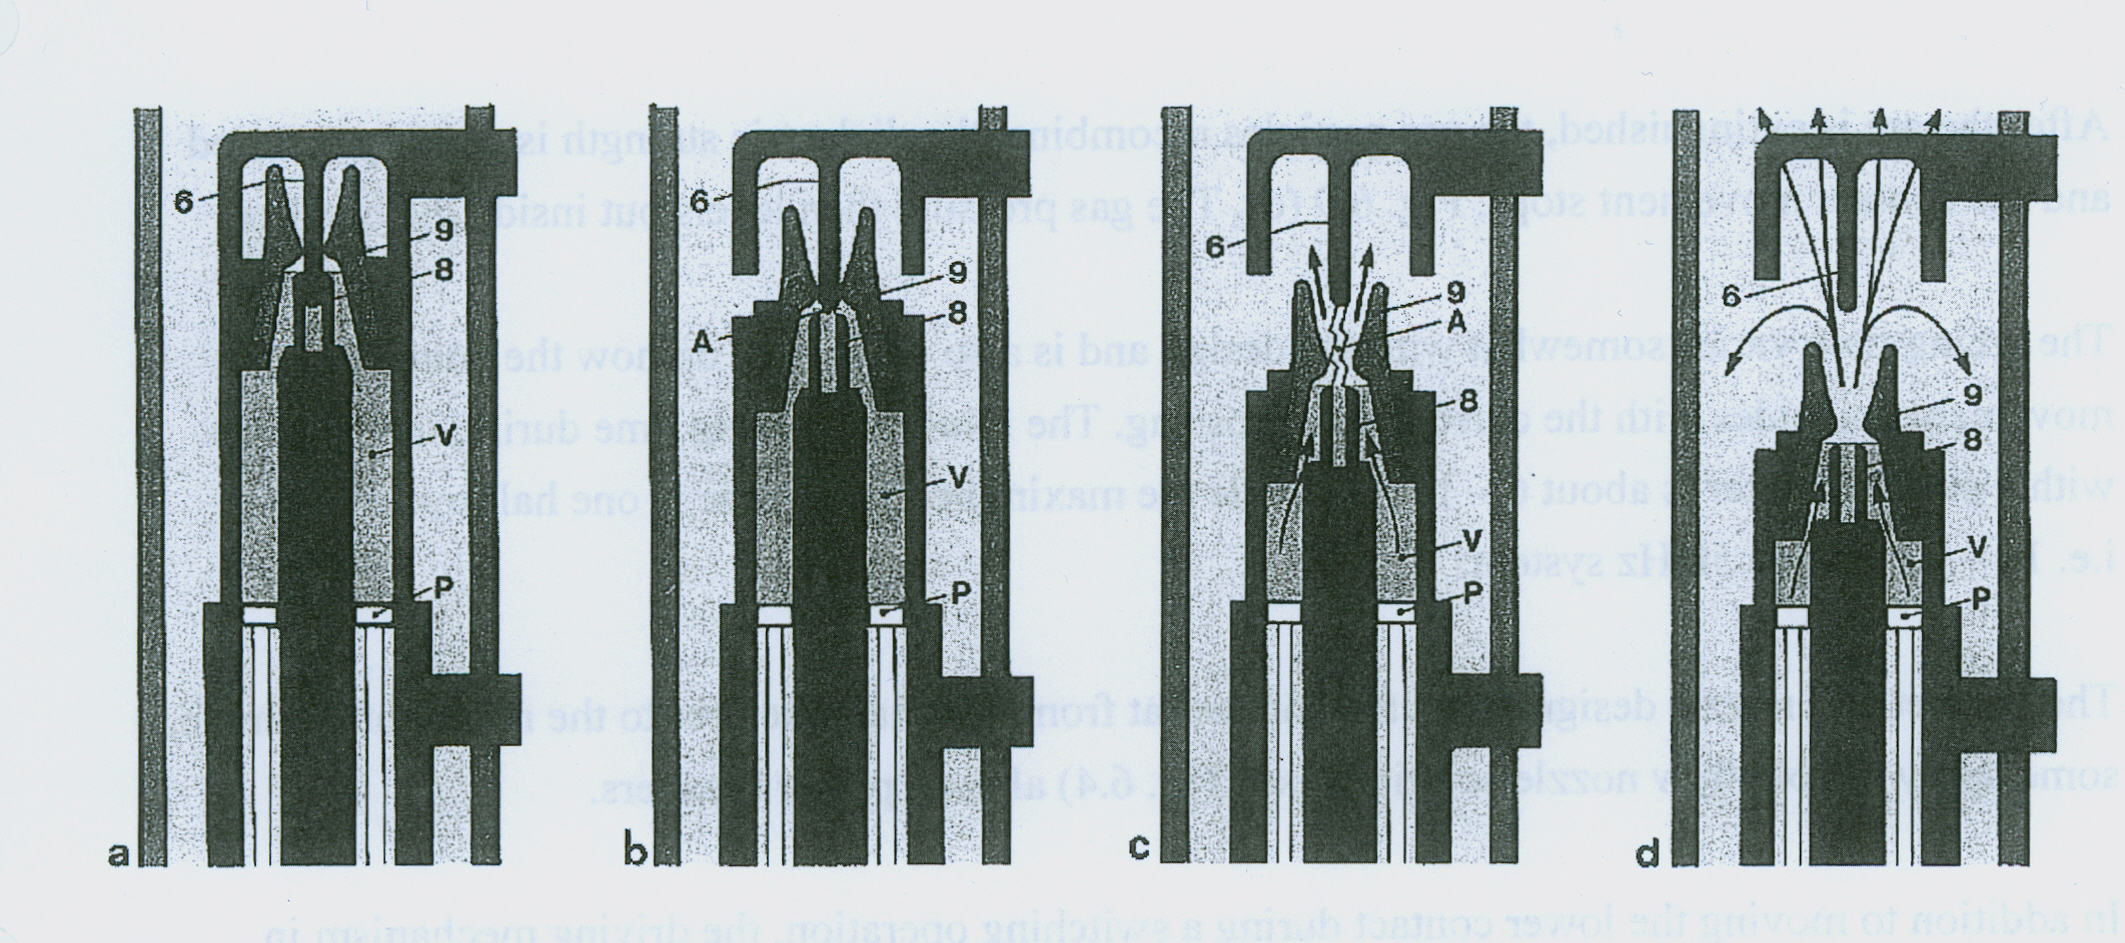
\includegraphics[scale=0.9]{Bilder/Theory/CircutBreakPuff1.png}
\caption{Interruption sequence in a breaker using the puffer mechanism \cite{bib:HVEbreak}.} \label{fig:CircutBreakPuff1}
\end{figure}

Figure \ref{fig:CircutBreakPuff1} displays a typical interruption sequence of breaker based on the puffer design. When the breaker is closed as seen in figure \ref{fig:CircutBreakPuff1}a, there is a gas volume \textit{(V)} trapped between the piston \textit{(P)} and the arcing contact \textit{(8)} and \textit{(6)}. At the moment the movable part of the arcing contact \textit{(8)} is pulled down, the volume decreases because of the fixed piston, and an increase in pressure due to compression of the gas occurs. Figure \ref{fig:CircutBreakPuff1}b illustrates that the main contact is open and that the current now only flows through the arcing contact.

The next stage of the interruption sequence is shown in figure \ref{fig:CircutBreakPuff1}c. The arcing contacts have now separated and an arc \textit{(A)} has ignited between the contacts. The pressurised gas that previously was trapped between the piston and the arcing contact is now released. The gas flow is guided by a nozzle \textit{(9)} that is fixed to the movable arcing contact. The gas flow will cool down the arc and blow away charge carriers between the contacts. If a sufficient gas flow is obtained, the arc will neither re-ignite after current zero nor extinguish before current zero.

The gas flow is partially dependent on the cross-section of the arc, which again is dependent on the current amplitude. A large current resulting in a large arc may block the hole in the nozzle, preventing a gas flow. This is called current clogging and may occur for certain nozzle designs at high current interruptions. In such an event, the pressure in the gas reservoir will increase further due to compression from mechanical moment of the arcing contact and thermal expansion in the gas because of heating from the arc. When the current amplitude approaches zero, its cross-section will decrease and the clogging effect will end. This will result in a powerful gas blast onto the arc, as indicated in figure \ref{fig:CircutBreakPuff1}d. For smaller current amplitudes, the arc cross-section is smaller and a clogging effect does not occur to the same extent. This generates a less intense gas flow, preventing the current to be interrupted before its natural zero crossing.

The self-blast, or third generation breaker, was developed with the goal of reducing mechanical power of the operating system, making it cheaper and less complex. Figure \ref{fig:selfBlast} illustrates the working principle of a breaker using self-blast to interrupt an arc. The difference between self-blast and puffer mechanism is that the puffer mechanism increases the pressure by reducing the volume, rather than the self-blast design which has a constant volume relying on a raise in temperature to increase the gas pressure \cite{bib:CBAC}. The self-blast design uses the heat generated from an arc burning between the arcing contacts to interrupt the current. The gas expands as it is heated by the burning arc. This increase in pressure leads to a gas flow on the arc, which cools it down, leading to the arc being quenched.

\begin{figure} [H]
\centering
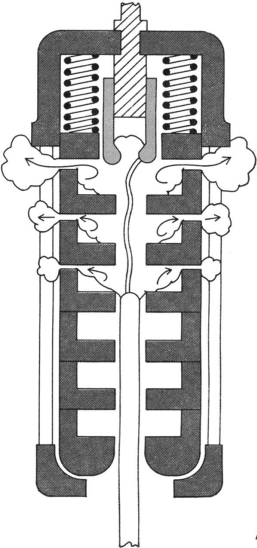
\includegraphics[scale=0.33]{Bilder/Theory/selfBlast.png}
\caption{Expulsion chamber in a breaker using the self-blast mechanism \cite{bib:CBAC}.} \label{fig:selfBlast}
\end{figure}

There are some disadvantages of the self-blast principle when compared to the puffer mechanism. The self-blast has a lower dielectric strength due to hot gas between the contacts after CZ. This gives a higher chance of re-ignition since hot gas has lower ionisation energy than cold gas. The design is also not well suited to break smaller currents. This is because the arc is less intense and therefore does not heat the gas sufficiently to create a strong enough blast. Therefore, it is common to combine self-blast and puffer mechanism in a hybrid design, so that it can handle both small and large currents. A compact LBS design using air as interrupting medium will probably rely on a puffer design. This is because of the small current an LBS is usually facing compared to a circuit breaker.

A good circuit breaker design is considered hard to develop, and the industry needs to optimise the product to meet the demands set by the market, like size and pressures. This is due to high short-circuit current, in the range of 40 kA and large recovery voltages. Because of this the industry has put a lot of effort into circuit breaker development. Nonetheless, when designing an LBS based on SF$_6$, it is common to take the working principle of a circuit breaker and scale it down to a suitable size for an LBS and then test it, and if it works the LBS might be sold on the market without further alterations. When using air, this development technique have not been used successfully, since higher demands are set to the interrupting capabilities of the switchgear. This is because SF$_6$ is superior to air as an interrupting medium and the behaviour of the arc also alters with the current. However, the same interruption techniques might be used but with more focus on optimisation. In figure \ref{fig:selfBlastandPuffer} the interrupter of a load break switch is shown. This is a down scaled version of a circuit breaker which has successfully been used to interrupt load current with SF$_6$ gas as interruption medium. 

\begin{figure} [H]
\centering
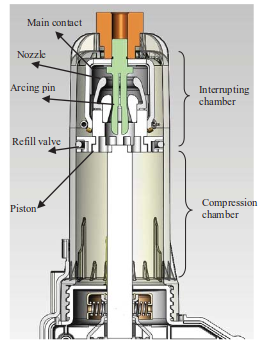
\includegraphics[scale=0.6]{Bilder/Theory/LBSselfblastandPuffer.png}
\caption{Schematic of a gas puffer interrupter \cite{bib:CBAC}.} \label{fig:selfBlastandPuffer}
\end{figure}

As can been seen in figure \ref{fig:selfBlastandPuffer} the load break switch features many of the same components as a circuit breaker, but the dimensions are scaled down. The interruption technique used is puffer based, and the operation sequence is as illustrated in figure \ref{fig:CircutBreakPuff1}. The article "Gas flow analysis in low energy arc puffer interrupters" presents an experiment where the the pressure in the pressure chamber of a LBS is measured during opening operation, and is then is simulated, so that a comparison of the theoretical and measured pressures can be presented. In figure \ref{fig:airPressurePuffer} the measured and simulated gas pressure from the paper, is shown during a cold gas opening operation, which means that the switch was unloaded during the test. As can be seen the measured pressure corresponds quite well, with the simulated pressure, when certain loss factors have been included in the simulation.


\begin{figure} [H]
\centering
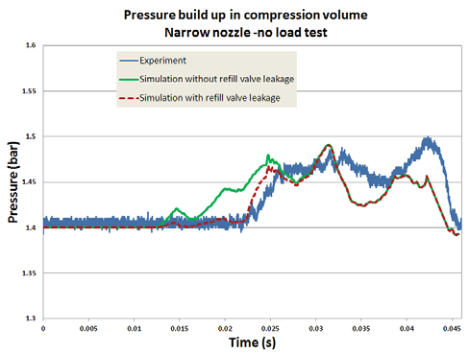
\includegraphics[scale=0.6]{Bilder/Theory/tankPressure.png}
\caption{Simulated pressure build up with different refill valve leakage settings compared to experimental results  \cite{bib:CBAC}.} \label{fig:airPressurePuffer}
\end{figure}

When introducing an arc to the system; the measured, and simulated pressures changes as shown in figure \ref{fig:airPressurePuffer2}. As seen in this figure, the pressure was not successfully simulated, and the difference between measured pressure, and simulation results are huge, and increases with a longer arcing time. This simulation technique have been used with success when simulating for circuit breakers. This gives reason to believe that the properties of the arc alters significantly when the current is reduced, as in a load break switch. Good simulation tools for air flows, when arcs like this is present, are still to be developed. Which makes scaling a circuit breaker down to a LBS without the possibility to know how the arc interacts with the gas flow hard, especially when using air as interruption medium and not SF$_6$.



\begin{figure} [H]
\centering
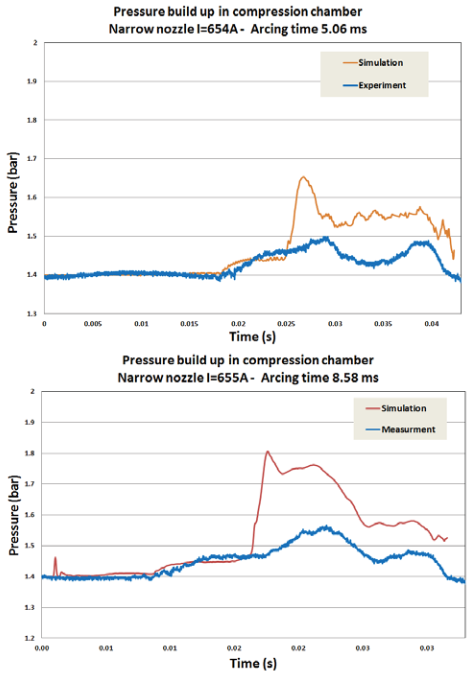
\includegraphics[scale=0.6]{Bilder/Theory/tankPressure2.png}
\caption{Pressure build up for load break tests with different arcing time   \cite{bib:CBAC}.} \label{fig:airPressurePuffer2}
\end{figure}

\subsection{Interrupting currents}
%As an interruption medium air is fairly good, and has been successfully used in the past to interrupt high currents at high voltages, some air-blast breakers are still in use. Dette hører kanskje inn i en innledning.
\subsubsection{Electrical conductivity in an arc} \label{sec:eleCondArc}
Gases have the ability to be good insulators as well as good conductors, mainly depending on the gas temperature. This is due to charged particles and electrons created by dissociation and ionisation of the molecules in the gas. Air is a mixture of several gases but might be simplified to consist mostly of nitrogen (N$_2$). In figure \ref{fig:condAir}, the electrical conductivity of air as a function of temperature can be observed.

\begin{figure}[H]
\centering
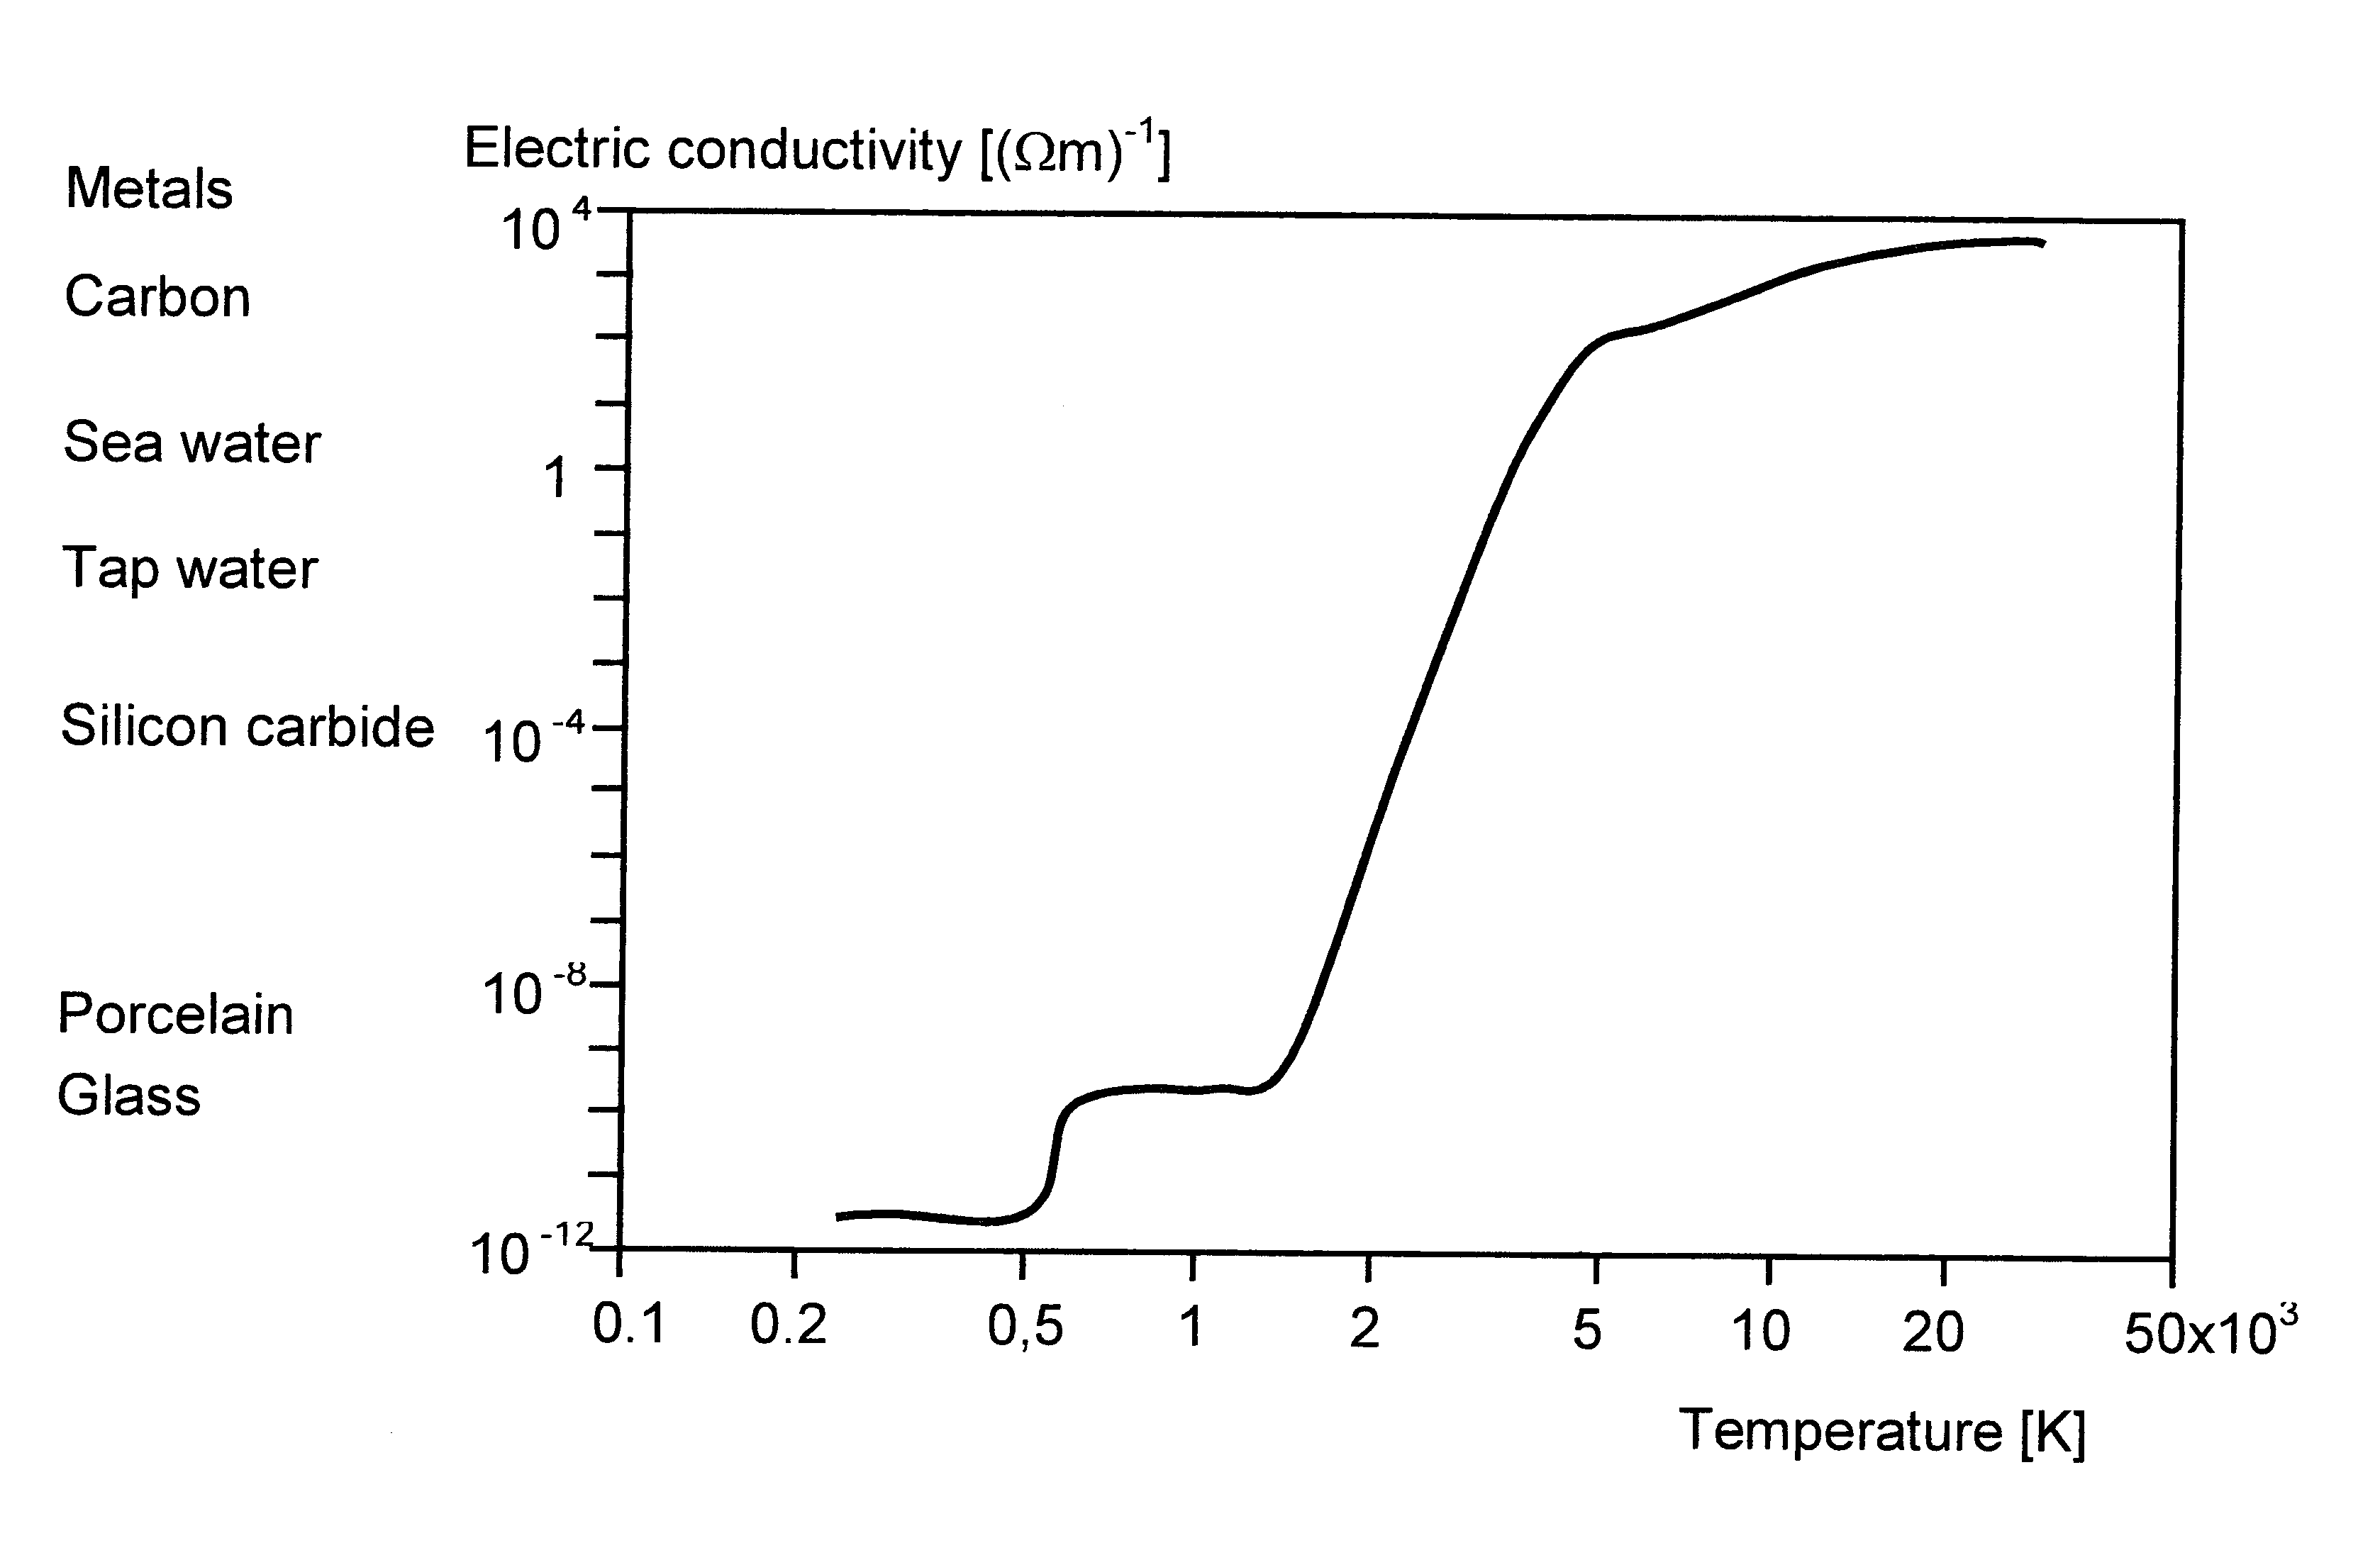
\includegraphics[scale=0.9]{Bilder/Theory/airConduct.png}
\caption{Electrical conductivity of air at atmospheric pressure \cite{bib:HVEbreak}.} \label{fig:condAir}
\end{figure}

The steep increase in conductivity can mainly be explained by the dissociation process and ionisation of N$_2$ due to temperature increase. The particle density of nitrogen as it dissociates due to high temperature in the gas is illustrated in figure \ref{fig:Ndensi}. When figure \ref{fig:Ndensi} is compared to figure \ref{fig:condAir}, a connection between temperature and the rapid decline of N$_2$, generation of the positive ion N$^+$, and the steep increase in conductivity of air is clearly presented.

\begin{figure}[H]
\centering
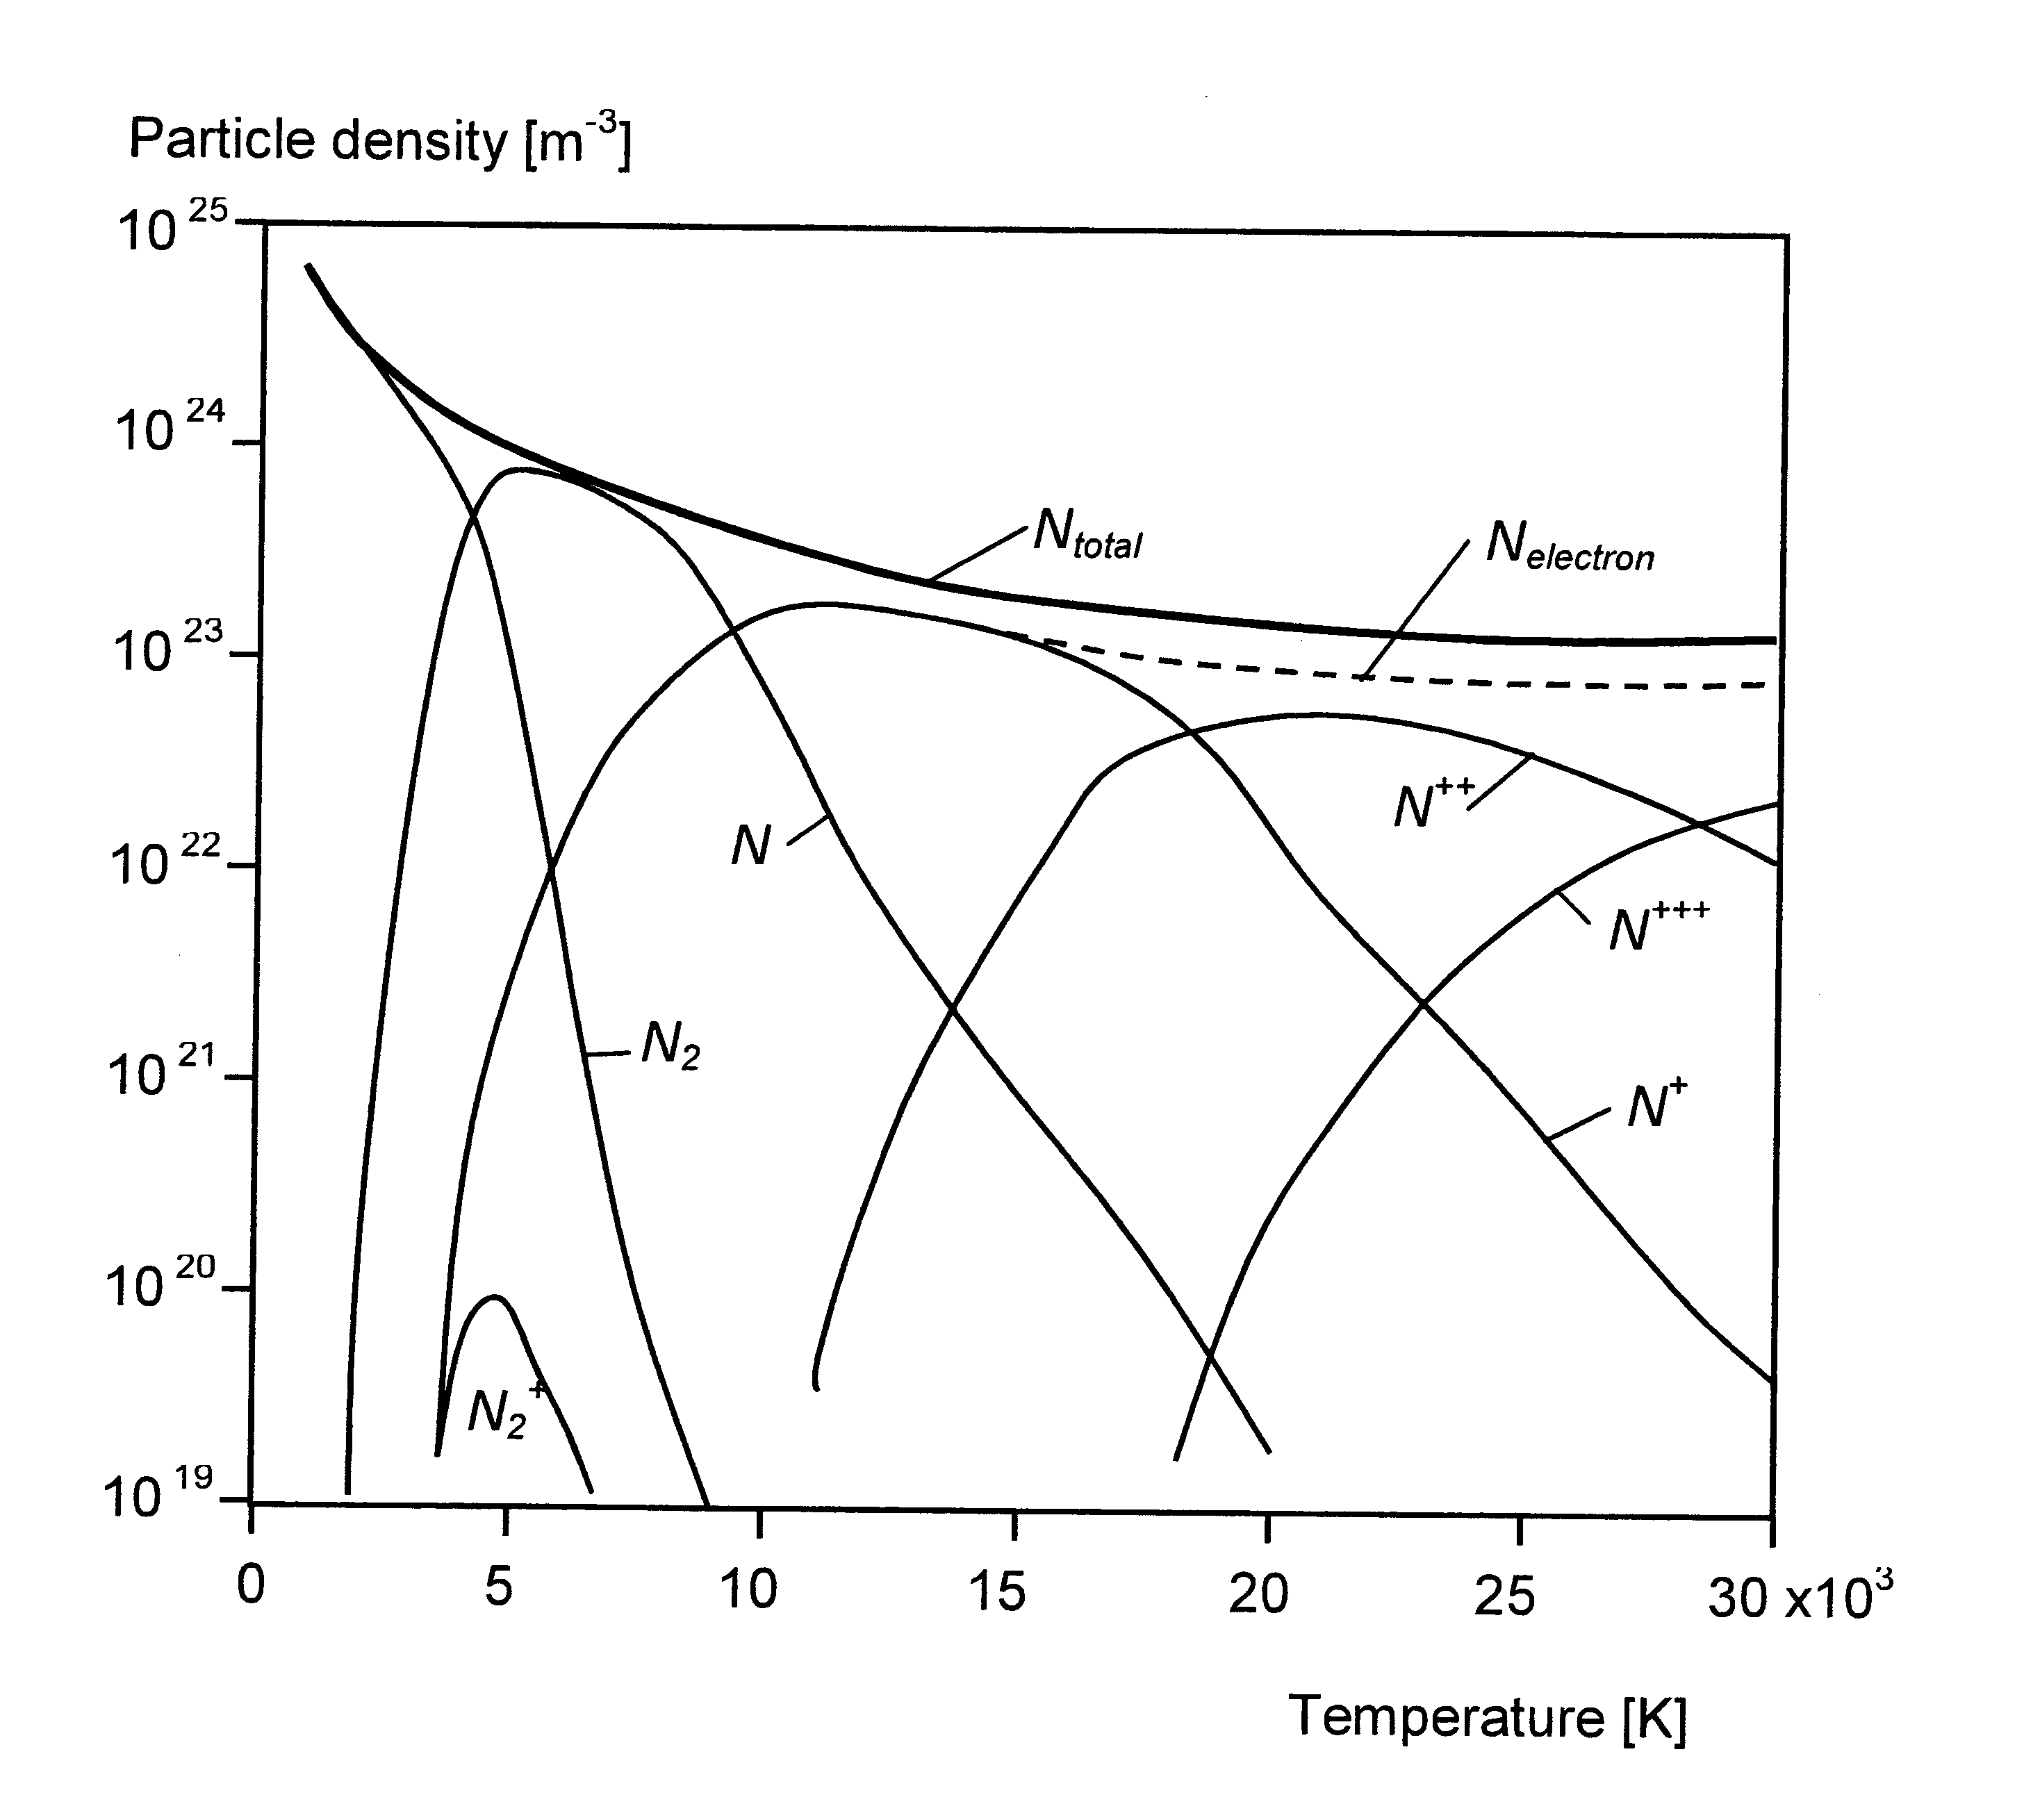
\includegraphics[scale=0.8]{Bilder/Theory/particleDensNit.png}
\caption{Particle density for different dissociation and ionisation products of nitrogen as a function of temperature \cite{bib:HVEbreak}.} \label{fig:Ndensi}
\end{figure}

Nitrogen is an electropositive gas, which means that it will have a tendency to give away electrons from its outer shell easily, especially when in a strong electric field and subjected to high temperatures. From figure \ref{fig:Ndensi}, the electropositive effect of N$_2$ is indicated via the generation of N$_{2}^{+}$ molecules. From table \ref{tab:thermalIonisation}, the thermal ionisation energy for some gases is presented. This points out that N$_2$ has a significant lower ionisation energy than SF$_6$, and it gives away electrons more easily.

\begin{table}[H]
\center
\caption{Thermal ionisation energy for some gases \cite{bib:HVEbreak}.}
\begin{tabular}{|l|c|c|}
\hline 
Particle type & Single ionisation [eV] & Double ionisation [eV] \\ 
\hline 
Air & 16.3 &  \\ 
\hline 
N$_2$ & 15.8 &  \\ 
\hline 
N & 14.5 & 44.1 \\ 
\hline 
O$_2$ & 12.5 &  \\ 
\hline 
SF$_6$ & 19.3 &  \\ 
\hline 
S & 10.4 & 33.8 \\ 
\hline 
F & 17.4 &  \\ 
\hline 
\end{tabular} 
\label{tab:thermalIonisation}
\end{table}

During a interruption sequence it is preferred to have different electrical conductivity depending on the current magnitude. When the current magnitude is high or raising, a good conductivity is needed. For most gases, including air this is obtained because the air is heated by the current travelling trough it, resulting in an high temperature and a good conductivity. This is important for an interruption medium as a low electrical resistance results in smaller losses, and therefore less heat generation of the surroundings. However, at the moment of CZ, and after; a fast transaction from a conducting to a insulating state of the interruption gas is important, as this will avoid a re-ignition of the arc. At this stage the interruption gas will use some time to recombine due to both cooling and relatively slow movement of the particles the gas consists of. In addition to this there will be free electrons in the contact gap, which increases the re-ignition chance. The oxygen in air is highly electronegative and will capture electrons. However, the concentration of oxygen is small relative to the concentration of nitrogen in air and this effect is therefore not very strong. Therefore a puffer is needed to blow away the charged particles and hot gas between the electrodes to avoid a re-ignition.

\subsubsection{Heat transportation in an arc} \label{sec:HeatTransport}
There are several different thermal conductive mechanisms in an electrical arc. The effects of these mechanisms vary with temperature, and therefore the heat transport in the arc is strongly dependent upon the temperature. In figure \ref{fig:tempConGas}, the thermal heat conductivity of several common interrupting gases is compared as a function of temperature.

\begin{figure}[H]
\centering
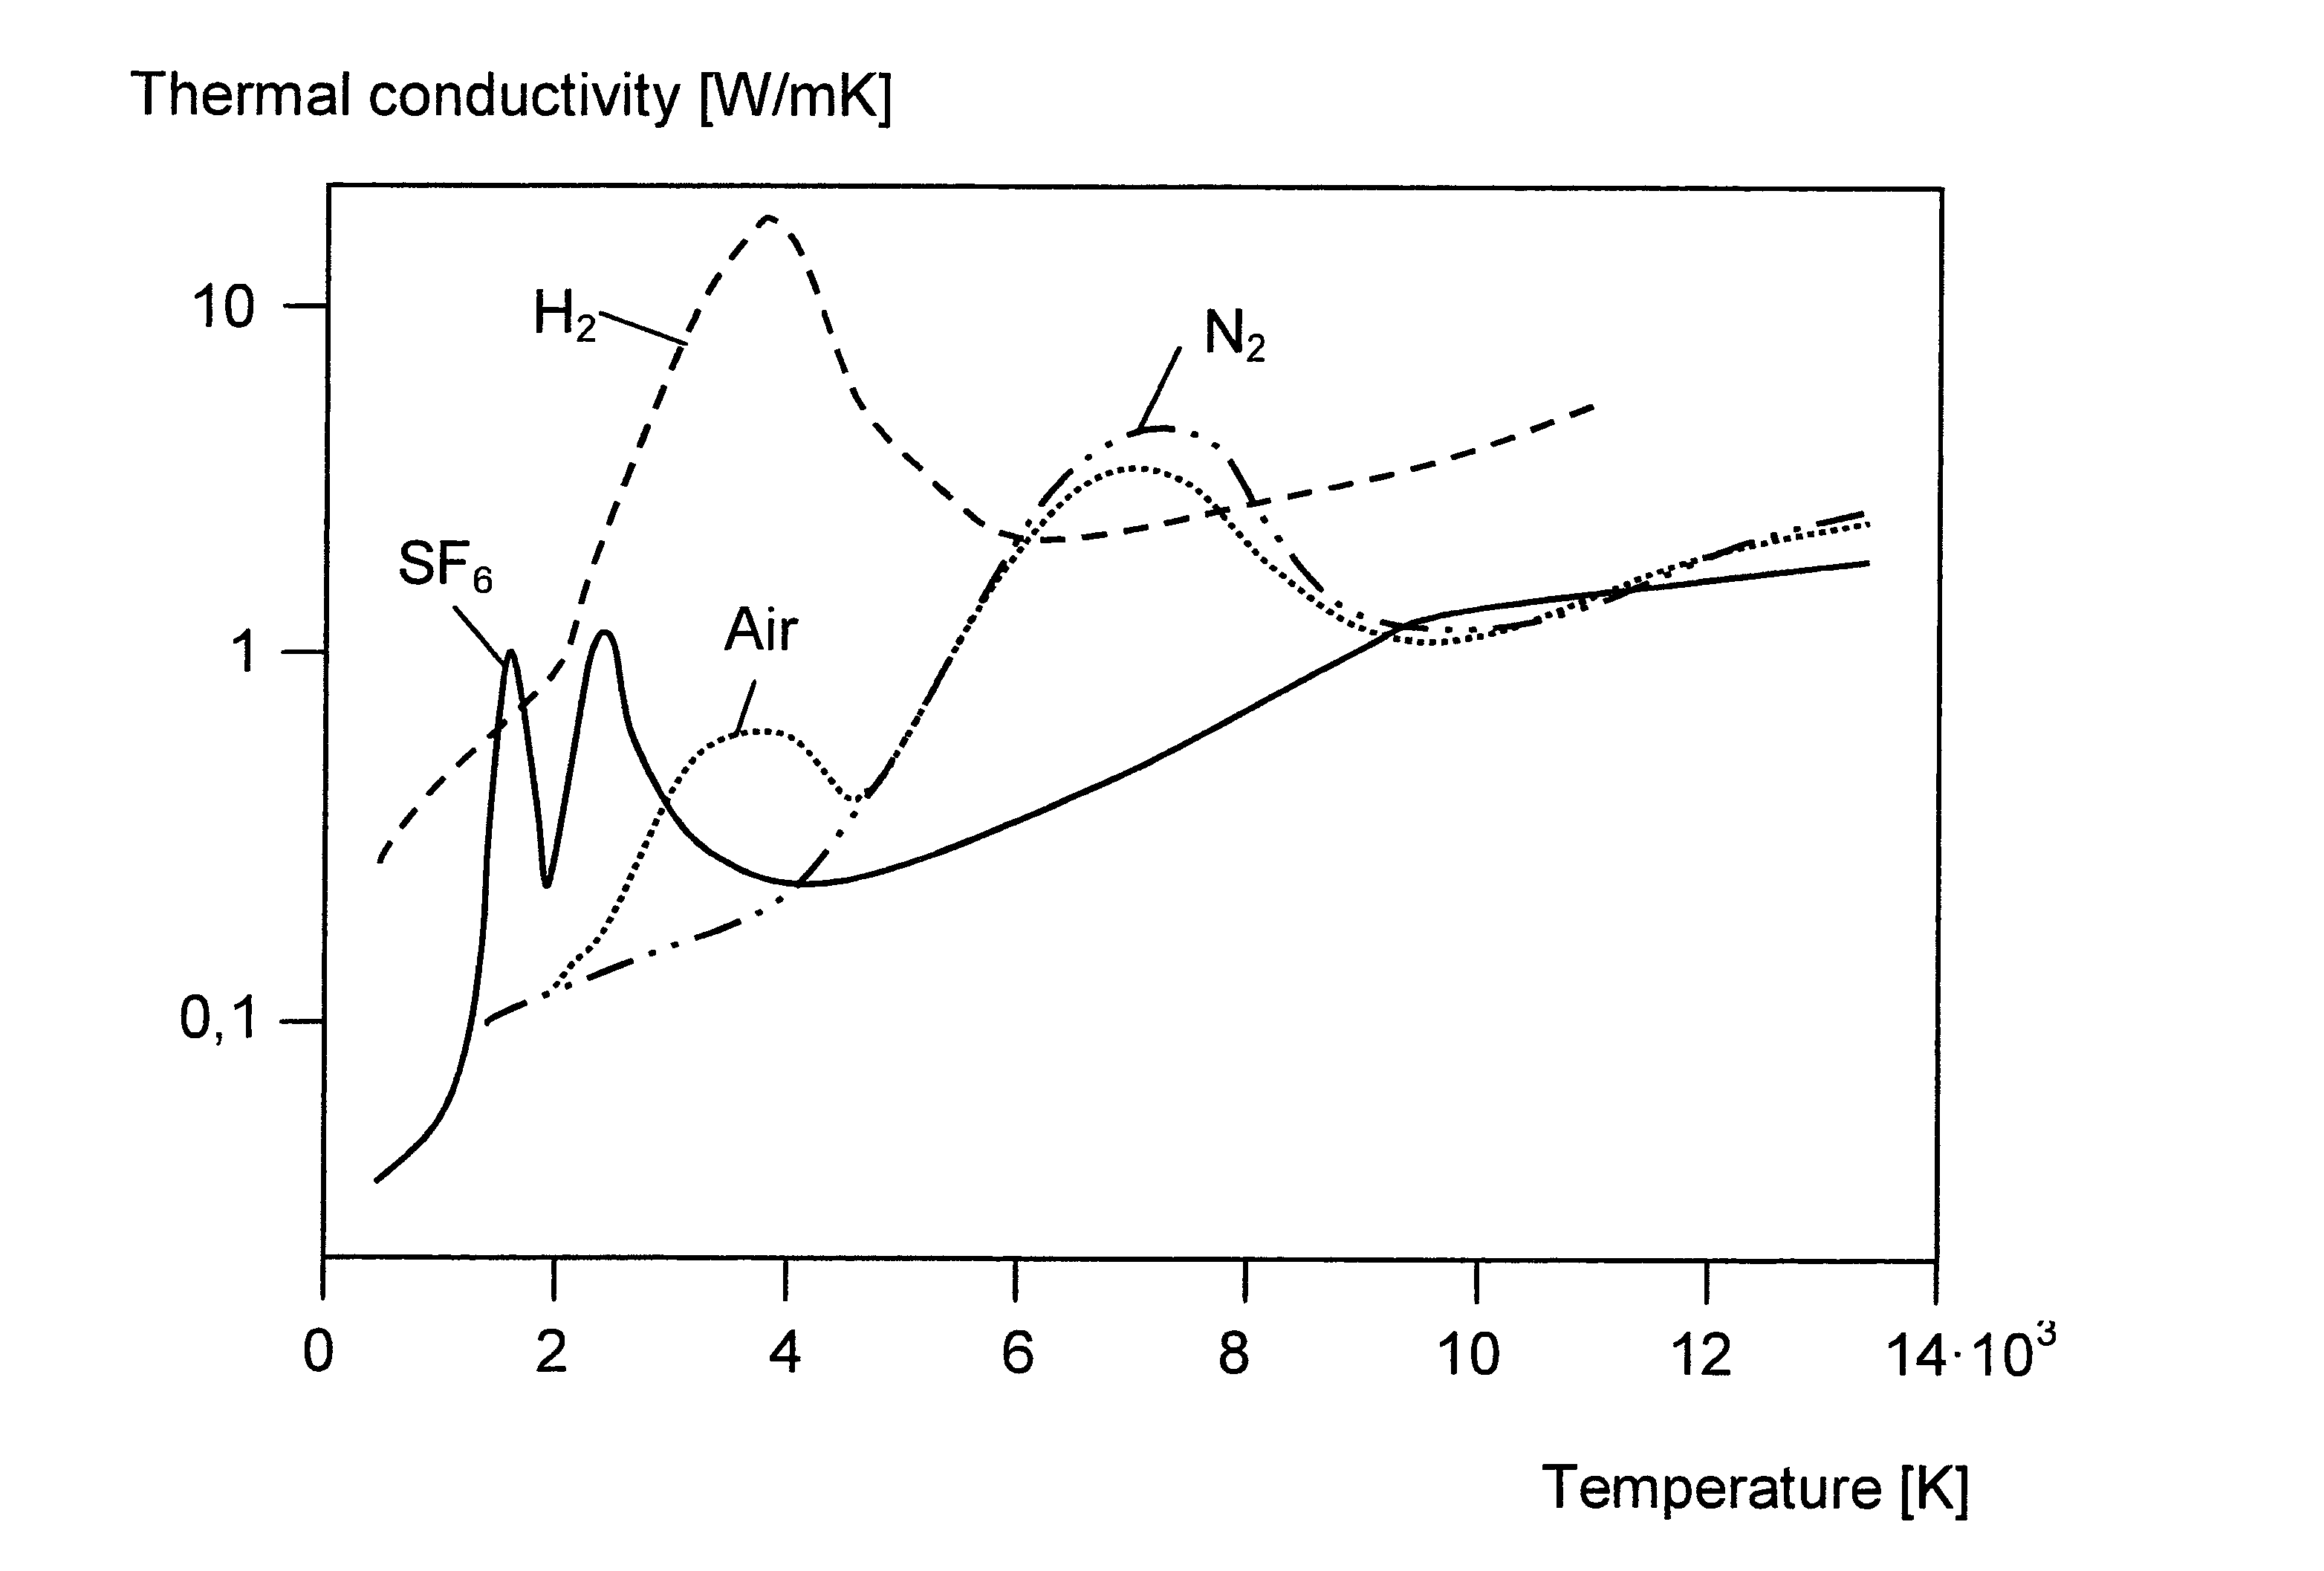
\includegraphics[scale=0.83]{Bilder/Theory/thermalCond.png}
\caption{Thermal conductivity as a function of temperature \cite{bib:HVEbreak}.} \label{fig:tempConGas}
\end{figure}

Due to the nature of the different stages in current interruption, it is desired that one uses a gas that has a thermal conductivity that suits the different stages right. When the current amplitude is rising, or is high, it is preferred that the thermal conductivity is low. This means that the plasma channel does not heat its surroundings but mainly keeps the dissipated energy stored in its core. This will result in a temperature rise in the plasma channel and a relatively small increase in the surroundings. As explained in section \ref{sec:eleCondArc}, a high arc temperature will result in high conductivity in the arc, which gives a low arcing voltage. If the thermal conductivity is high in this region, heating of the surrounding system will occur. This might result in a slower transaction between the conductive and insulating stage of the interrupting medium, due to the stored energy in the medium and the surroundings, resulting in a higher chance of re-ignition.

At the moment right before CZ, it is an advantage if the thermal conductivity of the gas is high. This will result in a fast cool-down time of the plasma channel since both the current amplitude is decreasing and the energy stored in the arc now is permitted out to its surroundings. A gas with high thermal conductivity in this stage of the interruption process will be able to recombine from an ionised and highly conductive to a non-conductive state fast, making it harder for a thermal re-ignition to occur. This is because of the quick cooling of the plasma channel. In gases where the thermal conductivity is low, the cooling mechanisms are of great importance, since a quick recombination of ionised gas does not occur in the same manner as when the medium is quickly cooled. Therefore, removal of hot gas and charge carriers must be done differently. This is described in detail in section \ref{sec:genDes}. The thermal conductivity profile of air is not well suited for current interruptions, at least if compared to the one of SF$_6$. If figure \ref{fig:tempConGas} is consulted it can be observed that air have a high conductivity when the temperature is high, and a low conductivity when the temperature is low. This is the opposite of the preferred characteristics. Even though air have a small peak in thermal conductivity between 3000 K and 4000 K, its thermal conductivity profile is regarded as one of the major challenges when using air as an interruption gas. 

The temperature distribution in a plasma channel can be divided into three sections \cite{bib:TDCIGBB}, as illustrated with figure \ref{fig:tempDist1}. Zone 1 is the highly conductive arc core and also the zone with the highest temperature. Zone 2 acts as an energy buffer during the decay of the arc while zone 3 is the cold gas surrounding the arc. When using cooling-mechanisms to quench the arc, it is primarily the second zone of the temperature profile that is cooled. The first zone's temperature will mainly be dependent on the current passing through the arc and will not be influenced by the cooling mechanism in the same degree. If the cooling is sufficient, the energy stored in zone 2 when the arc approaches CZ is low and therefore its effect as an energy buffer is reduced, resulting in a rapid decline in temperature in the arc core as the current approaches zero. This makes the interrupting medium's ability to transport energy important when investigating efficient cooling methods. As figure \ref{fig:tempConGas} has pointed out, SF$_6$ has the ability to transfer heat between zone 1 and 2 fast in the right temperature range compared to the interrupting sequence. Air has to a lesser degree the ability to do this.

\begin{figure}[H]
\centering
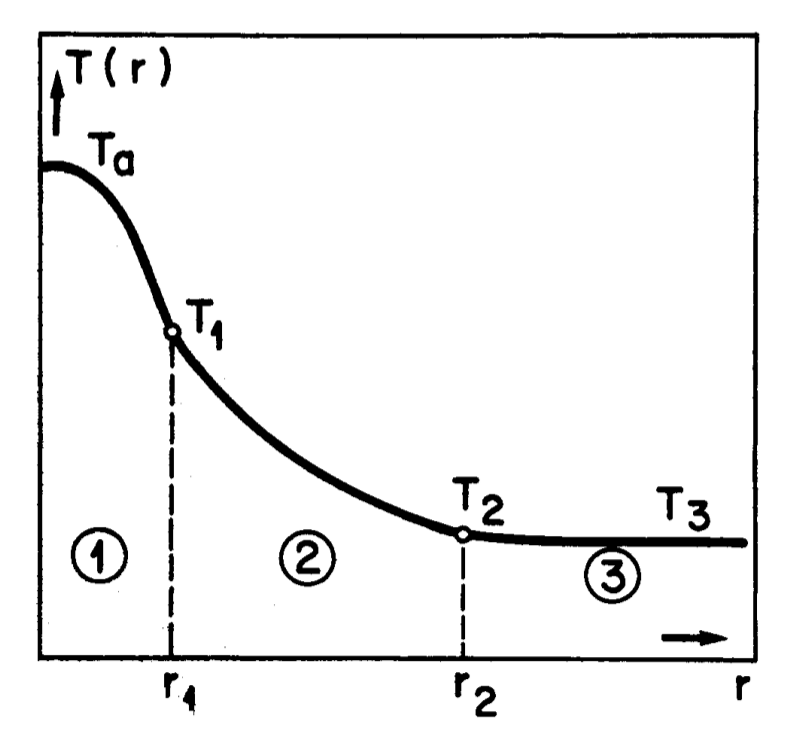
\includegraphics[scale=0.25]{Bilder/Theory/tempZonesArc.png}
\caption{Radial temperature distribution in a plasma channel \cite{bib:TDCIGBB}.} \label{fig:tempDist1}
\end{figure}

In figure \ref{fig:tempDist2}, shows how the temperature distribution varies with the electrical current. Due to radiation losses in the arc, the temperature has a upper limit of about 20 000 K to 30 000 K. At this point the cross-section of the arc will increase rather than the temperature \cite{bib:HVEbreak}. However, it is not common for an LBS to experience these temperature ranges, and its temperature distribution will mainly be in the lower current part of the figure.

\begin{figure}[H]
\centering
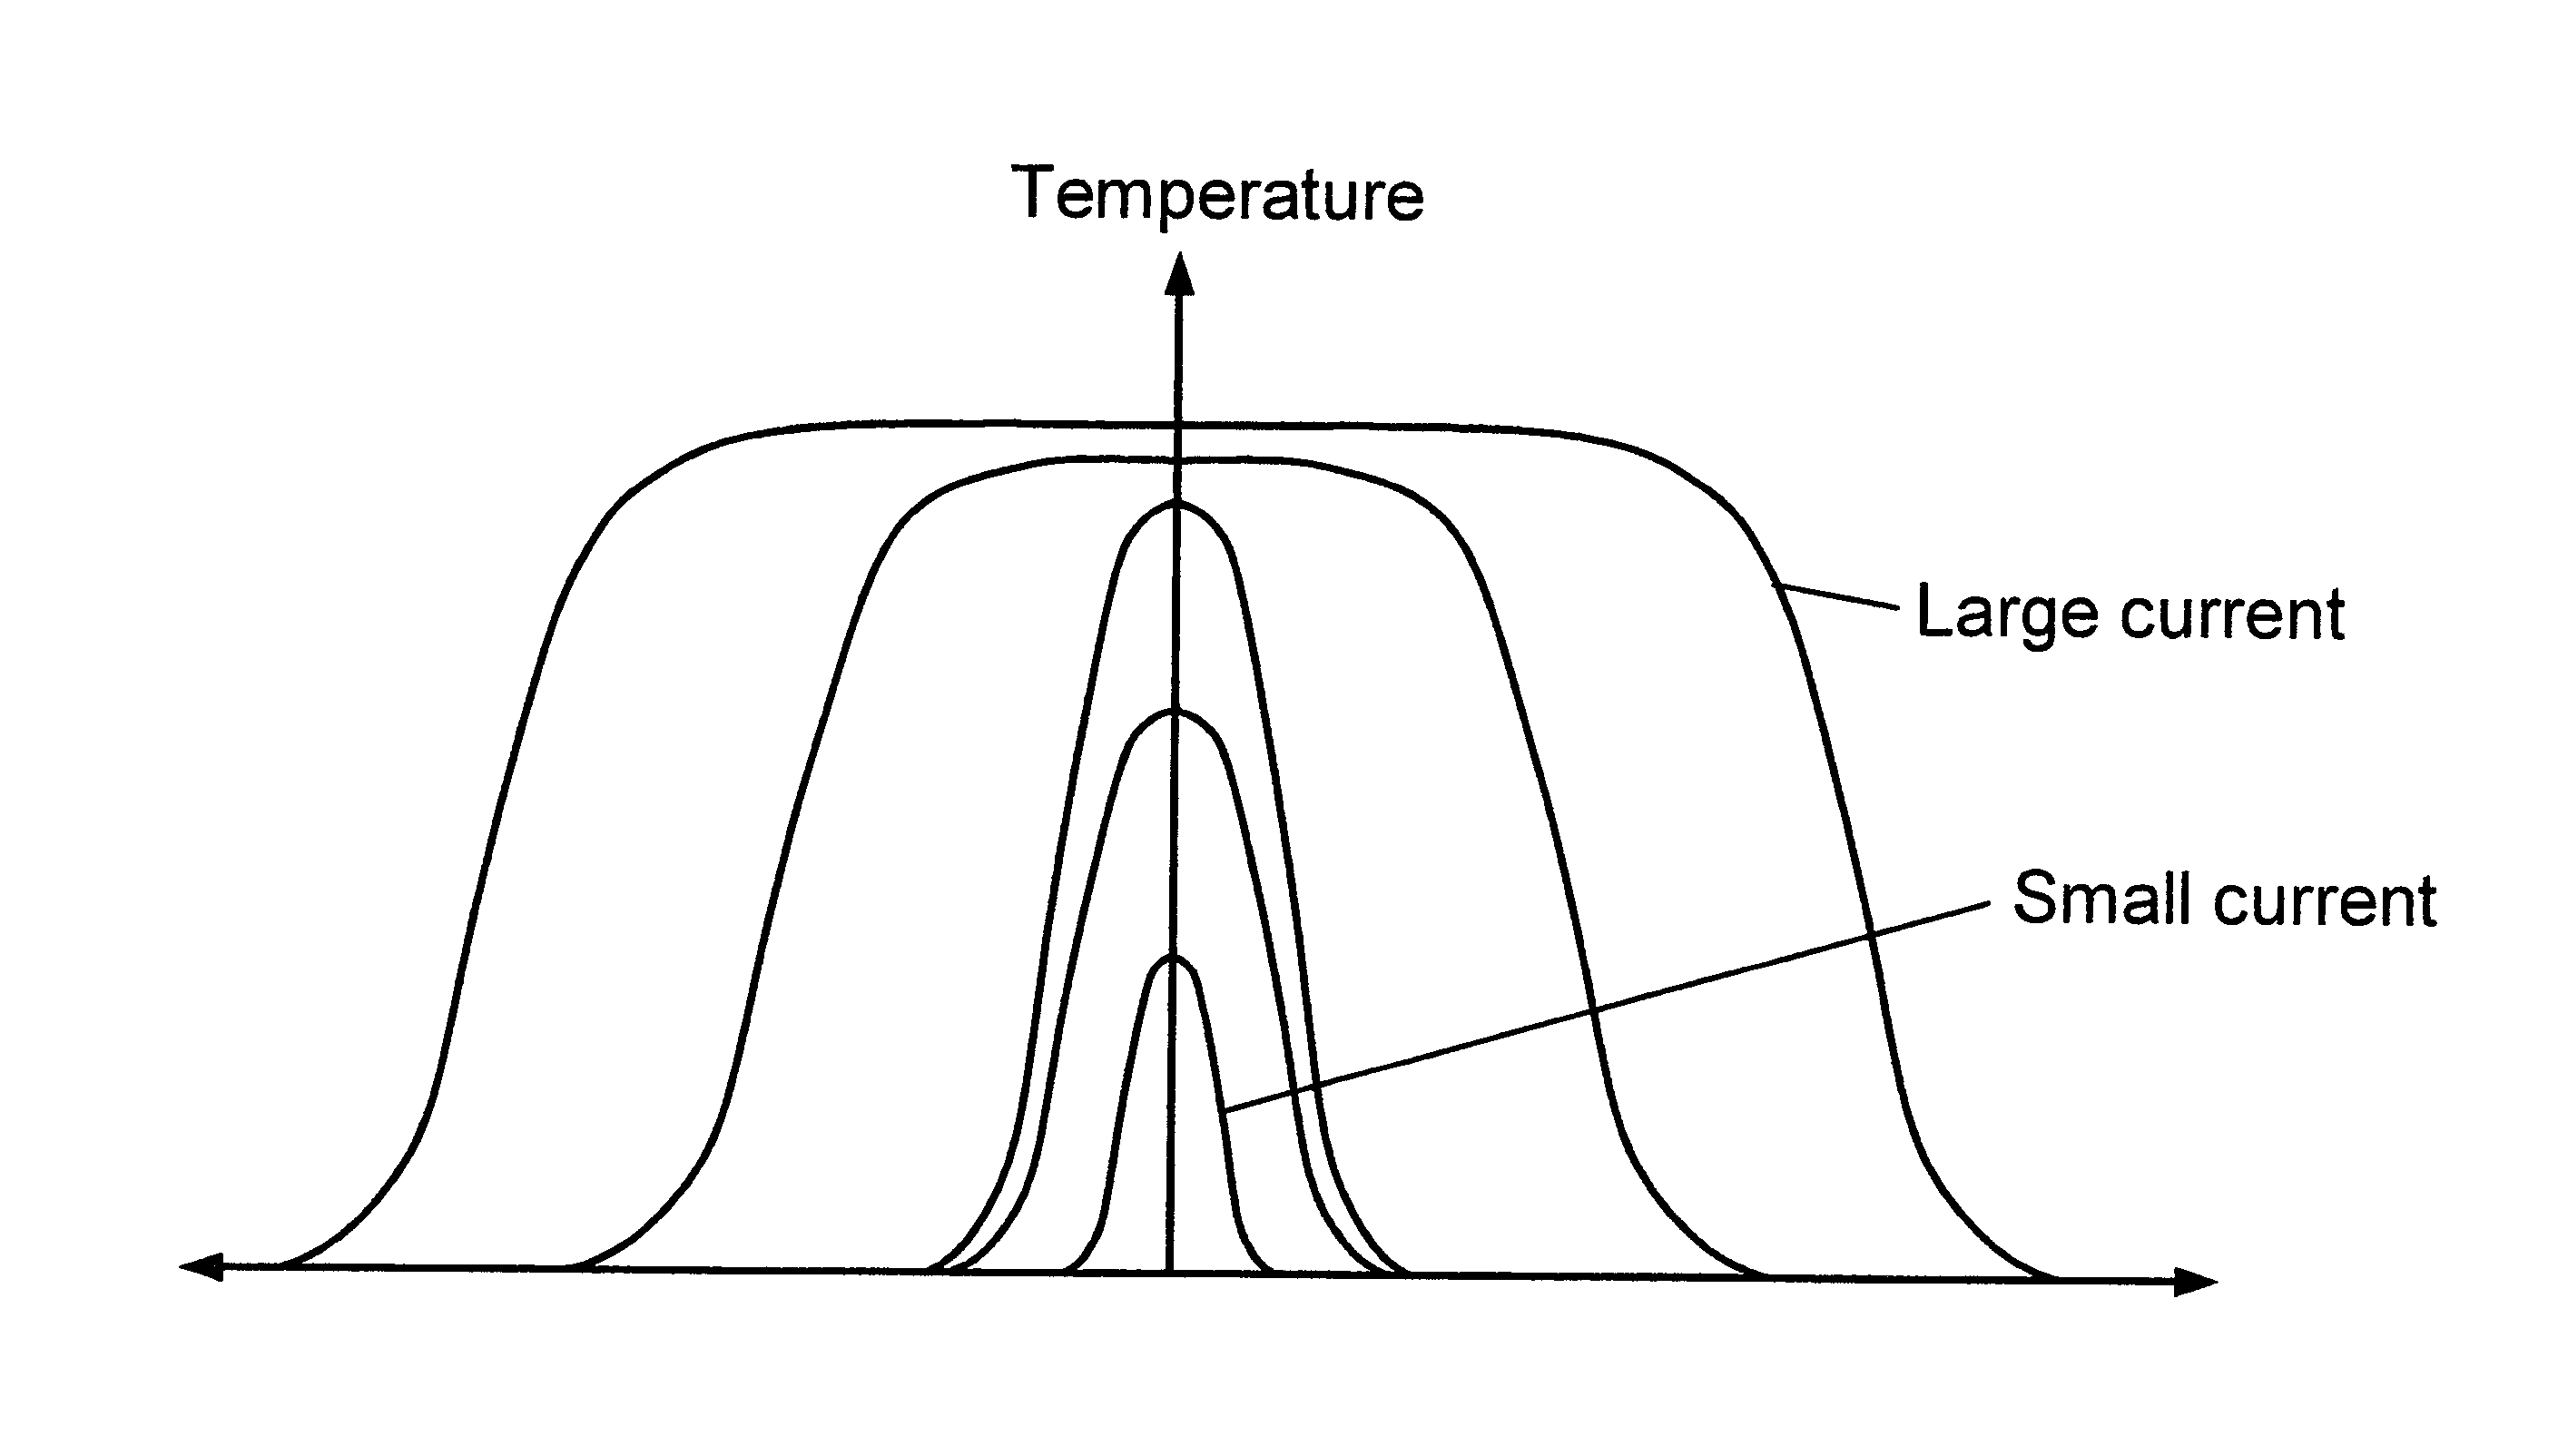
\includegraphics[scale=0.85]{Bilder/Theory/plasmaChannel1.png}
\caption{The radial temperature distribution in a plasma channel for different current magnitudes \cite{bib:HVEbreak}.} \label{fig:tempDist2}
\end{figure}

\cleardoublepage

\section{Method}

\subsection{Test circuit} \label{sec:testCir}

Figure \ref{fig:testSwitchRiggEq} illustrates the physical appearance of the test switch. The numbered parts are: 1. Compressed air reservoir (connected to the high voltage supply circuit), 2. Tulip contact, 3. Nozzle, 4. Pin contact, 5. Connection to load circuit, 6. Spring drive mechanism, 7. Electromagnet release mechanism, and 8. Position transducer.

\begin{figure} [H]
\centering
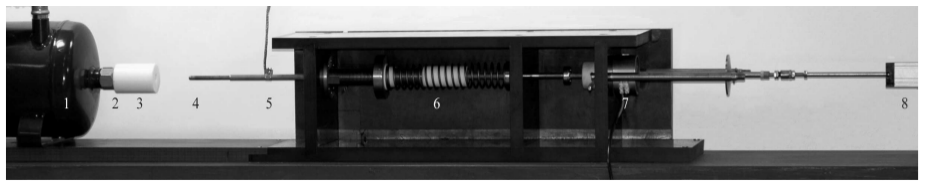
\includegraphics[scale=0.5]{Bilder/Method/switchTest.png}
\caption{The physical appearance of the test switch \cite{bib:AFIMVLBA}.} \label{fig:testSwitchRiggEq}
\end{figure}

Figure \ref{fig:testCurcuit} displays the laboratory test circuit used for the interruption tests. The circuit is designed to supply a 50 Hz / 13.8 kV current. It is possible to shape the transient recovery voltage (TRV) by tuning the parameters L$_1$, L$_s$, R$_1$, R$_d$, and C. The systems' short circuit parameters are R$_{sc}$ and L$_{sc}$. The TRV generated during interruption is set to simulate the standard for a 24 kV / 630 A class from the International Electrotechnical Commission (IEC), which corresponds to:

\begin{itemize}
\item The initial part of the TRV has a rate of rise in recovery voltage (RRRV) of 71 - 73 V / $\mu$s.
	\begin{itemize}
		\item The voltage difference is measured over the first 20 $\mu$s after CZ.
	\end{itemize}
\item The first voltage peak is between 7.0 and 7.4 kV, with a rise time of approximately 96 $\mu$s.
\end{itemize}

\begin{figure} [H]
\centering
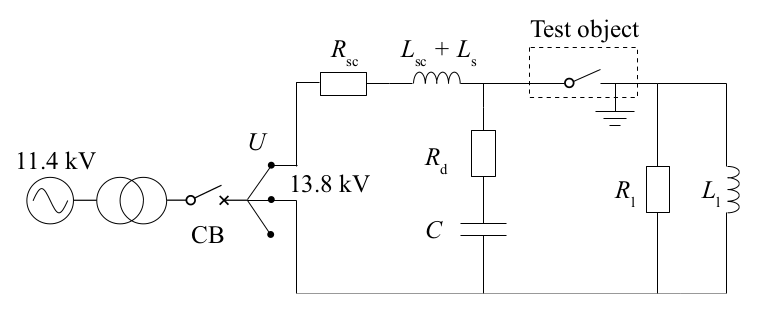
\includegraphics[scale=0.35]{Bilder/Method/circuit.png}
\caption{Circuit used for the interruption test \cite{bib:AFIMVLBA}.} \label{fig:testCurcuit}
\end{figure}

In table \ref{tab:testParameters}, the values of the different test circuit parameters and the corresponding currents can be observed. The test is conducted at currents with an RMS value of 630 A and 880 A. In the entire experiment, the TRV is kept constant up to and including the first voltage peak. In the case of a failed interruption, a thermal re-ignition occurs within a few microseconds after CZ.

\begin{table}[H]
\center
\caption{Circuit parameters and resulting currents \cite{bib:AFIMVLBA}. }
\begin{tabular}{|c|c|c|c|c|c|}
\hline 
L$_s$ [mH] & L$_1$ [mH] & R$_1$ [$\Omega$] & C [nF] & R$_{d}$ [$\Omega$] & I [A] \\ 
\hline 
6.9 & 86.2 & 22.1 & 102 & 198 & 630 \\ 
\hline
2.9 & 60.2 & 15.1 & 156 & 170 & 880 \\
\hline   
\end{tabular} 
\label{tab:testParameters}
\end{table}

A resistive transducer is measuring the contact position, while a Hall Effect current transducer is measuring the current through the test switch. The voltage between the contacts is measured with a parallel resistive / capacitive voltage divider. All measurements are transmitted through optical fibres to a 12 bit resolution transient recorder with a sampling frequency of 2.5 MHz. The pressure in the tank is only measured before each test with an accuracy of 0.01 bar.

\subsection{The switch and contact geometry}
This experiment is conducted using copper-tungsten arcing contacts, polytetraflourelthylene (PTFE) nozzles, and air as interrupting medium. It is an open system, with the surrounding air at atmospheric pressure \textit{p$_0$} and a six-litre tank with a pre-filled upstream overpressure \textit{p$_u$}, used during the interruption process to quench the arc. It is possible to adjust the upstream pressure, contact speed, and position at current zero (CZ) independently, as well as the contact and nozzle geometry. The current and TRV can be changed by changing the parameters of the laboratory test circuit, as described in section \ref{sec:testCir}.


A simple drawing of the contact and nozzle is displayed in figure \ref{fig:contactAndNozzle}. The length of the nozzle is 20 mm, and the inner diameter is \textit{D}. Axial symmetry is present along the x-axis. Two different contact geometries are going to be tested, denoted a and b. The dimensions of the different geometries are given in table \ref{tab:contGeoPara}, and the definitions of the different areas are illustrated in figure \ref{fig:AreacontactAndNozzle}. The angle $\mathrm{\theta}$ is defined so that $A_\mathrm{{funnel}}=4 \cdot A_\mathrm{{nozzle}}$ for each geometry.

The contact position \textit{x} is defined as the axial distance between the tulip and the pin contact. At starting position, \textit{x}= -60 mm, and the pin contact is acting as a plug for the tank. This makes it possible to pre-set an upstream pressure. The contact is held in place by an electromagnet, and is set to motion when the magnet releases a compressed spring. The spring accelerates the pin contact up to a speed of approximately 5.5 m/s at \textit{x}=0. At this position, the spring is unloaded and the pin moves with a constant speed until the contact is fully open at \textit{x}=110 mm.

\begin{figure} [h]
\centering
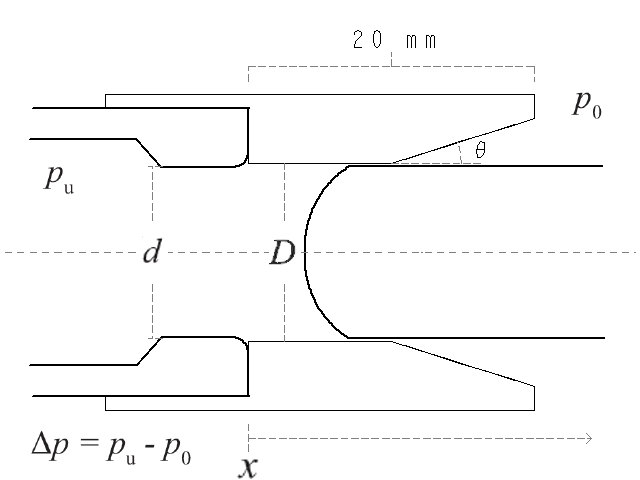
\includegraphics[scale=0.45]{Bilder/Method/ContactAndNozzleFunnelShape5.png}
\caption{The contact and nozzle. The diameter of the contact is \textit{d}, and the inner diameter of the nozzle is \textit{D}.} \label{fig:contactAndNozzle}
\end{figure}

\begin{figure} [H] %denne må byttes ut.
\centering
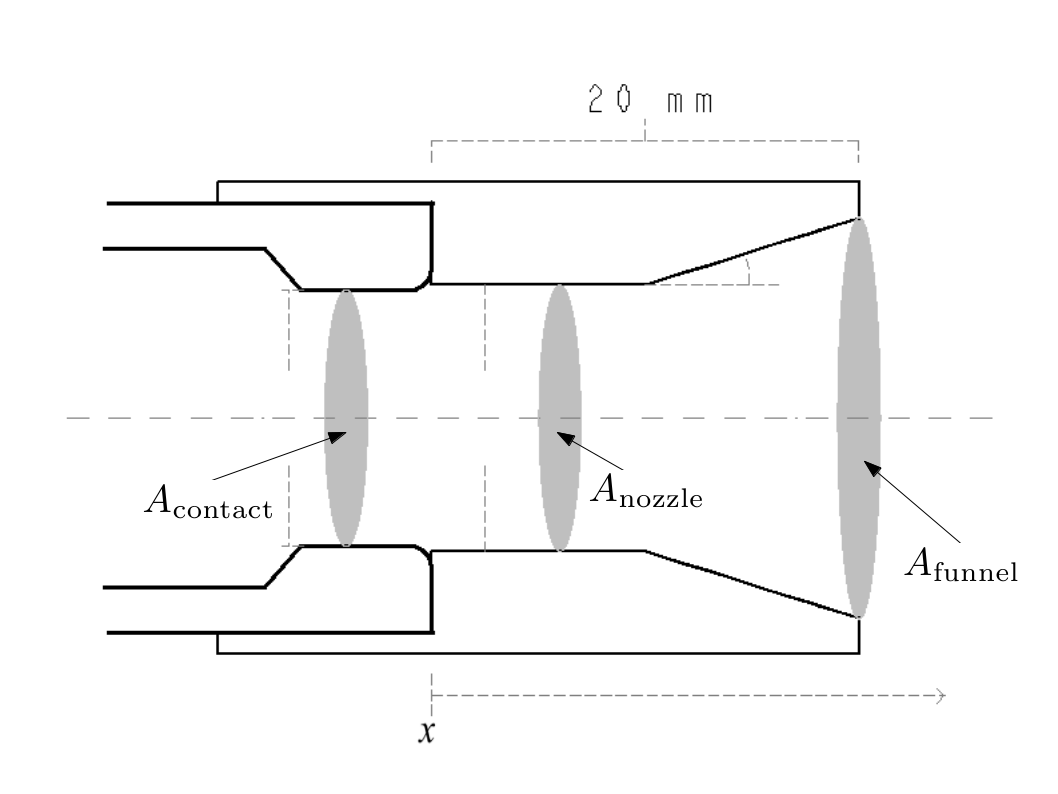
\includegraphics[scale=0.35]{Bilder/Method/AreaDef.png}
\caption{Overview of the definitions of the areas.} \label{fig:AreacontactAndNozzle}
\end{figure}

\newpage
\begin{itemize}
\item $A_\mathrm{{contact}}$ is the cross section of the contact pin, as well as the area of the tulip contact. The area is described by equation \eqref{eq:A_contact}.

\item $A_\mathrm{{nozzle}}$ is defined as the area of the cylindrical part of the nozzle, where x=[0,10] mm. The area is described by equation \eqref{eq:A_nozzle}.

\item $A_\mathrm{{funnel}}$ is defined as the area at the end of the nozzle, where x=20 mm, and the diameter of the funnel is at its largest. This area is described by equation \eqref{eq:A_funnel}.

\item $A_\mathrm{{ring}}$ is in table \ref{tab:contGeoPara} defined as the area between the pin contact and the cylindrical part of the nozzle, where x=[0,10] mm, and is described by equation \eqref{eq:A_ring_1}. For x=[10,20] mm, $A_\mathrm{{ring}}$ is a function of the pin's position, x, inside the nozzle, described by equation \eqref{eq:A_ring_2}.
\end{itemize}

\begin{equation} \label{eq:A_contact}
A_\mathrm{{contact}}=A_\mathrm{{tulip}}=\pi \frac{d^2}{4}
\end{equation}
\begin{equation} \label{eq:A_nozzle}
A_\mathrm{{nozzle}}=\pi \frac{D^2}{4}
\end{equation}

\begin{equation} \label{eq:A_funnel}
A_\mathrm{{funnel}}=4 \cdot A_\mathrm{{nozzle}}=4\pi \frac{D^2}{4}
\end{equation}

\begin{equation} \label{eq:A_ring_1}
A_\mathrm{{ring}}=A_\mathrm{{nozzle}}-A_\mathrm{{contact}}=\pi\left( \frac{D^2}{4}-\frac{D^2}{4}\right)
\end{equation}
\begin{equation} \label{eq:A_ring_2}
A_\mathrm{{ring}}(x)=\pi\left( \left(\frac{10-x}{\sin (\theta)}+\frac{D}{2}\right)^2-\frac{D^2}{4}\right)
\end{equation}

\begin{table}[H]
\center
\caption{Contact geometry parameters.}
 \begin{tabular}{|c|c|c|c|c|c|c|c|c|}
\hline 
Geometry & D [mm] & d [mm] & $\frac{D}{d}$ & $\mathrm{\theta}$ & $A_\mathrm{{contact}}$ [mm$^2$] & $A_\mathrm{{ring}}$ [mm$^2$] & $A_\mathrm{{nozzle}}$ [mm$^2$] & $A_\mathrm{{funnel}}$ [mm$^2$]\\ 
\hline 
a & 6.25 & 6.0 & 1.04 & 17.4 & 28.3 & 2.4 & 30.7 & 122.8\\ 
\hline 
b & 7.40 & 7.0 & 1.06 & 20.3 & 38.5 & 4.5 & 43.0 & 172.0\\ 
\hline 
\end{tabular} 
\label{tab:contGeoPara}
\end{table}

\newpage
\subsection{Procedure}
Interruption tests with CZ occurring both inside and outside the nozzle are carried out. Four tests in total are conducted in this interruption experiment. One test consists of one contact geometry at a current magnitude of either 630 A or 880 A with a minimum of five interruptions inside the funnel part of the nozzle and five interruptions outside the nozzle at each pressure level. At least three different pressure levels are included in each test. Both the first and second CZ are included in this study in order to provide as much data as possible.

"Inside funnel" is defined as contact position x = [10, 20] mm and "outside nozzle" as x = [20, 60] mm at first CZ. Results from zero crossings that occurs in the cylindrical part of the nozzle, x $<$ 10 mm, between the tulip contact and the start of the funnel-shaped nozzle are discarded. The first CZ occurs within x $<$ 60 mm, and the second CZ occurs for x $>$ 60 mm, as the contact speed during all tests is 5.5 mm/ms $\pm$ 0.5 mm/ms. When testing the interrupting capabilities inside the funnel, the first CZ is aimed to occur at x=15 mm, and when testing outside the nozzle, the first CZ is aimed at x=30 mm. Due to variation in the travelling speed of the contacts, some difference in the position of the pin at the moment of CZ will occur between each interruption attempt.

When testing the interrupting capabilities, the test procedure for each of the four cases is as follows: 

\begin{itemize}
\item[1.] A pressure level that seems to be in the area of interest is found by performing some initial test interruptions at different pressure levels. This level is kept constant for at least five interruption tests.
\item[2.] If a pressure level results in less than 100\% successful interruptions, at least five new tests with a higher upstream pressure (next level) are conducted. This is repeated until at least one pressure level with five successful interruptions is found.
\item[3.] Then, the pressure is stepped down until 60\% or more of the interruption attempts fail, or the lowest possible pressure level is tested.
\end{itemize}

When testing for variations in the arcing voltage between a successful and unsuccessful interruption, a pressure level where the interruption success rate is 50 \% is used. Then, five successful interruptions and five unsuccessful interruptions are obtained while the arcing voltage is measured and stored for further use. All the interruptions should occur outside the nozzle. The switching process is filmed by a high-speed camera so that the path of the arc can be monitored during the interruption.

The pin is cleaned, polished, and greased between each test to ensure a smooth surface. The contacts and nozzle are replaced regularly to avoid contact wear and nozzle deformation. This is to ensure that the geometry is constant through the whole experiment.
\cleardoublepage

\section{Results}
\subsection{Interruption tests} 


\newpage
\subsection{Arcing voltage}


\newpage
\subsection{Durability of the arcing contacts} \label{sec:durability}



\cleardoublepage

\section{Discussion}
\subsection{The probability of interruption} 


\subsection{Arcing voltage considerations}
 

\subsection{Durability of the arcing contacts} \label{fig:durability}


\newpage
\subsection{Suggestion for further work}
\subsubsection{A nozzle that minimises arc impact on air flow}


\subsubsection{Cone-shaped nozzle}


\cleardoublepage

\section{Conclusion}


\cleardoublepage
\begin{thebibliography}{10}
\bibitem{bib:SF6PI} L.G. Christophorou, J. K. Olthoff, and R.J. Van Brunt, "Sulfur hexafluoride and the electric power industry", \textit{IEEE Electrical Insulation Magazine, vol. 13, No. 5, pp. 20-24}, Oct. 1997.

\bibitem{bib:comSub} amesimpex.com, \url{http://www.amesimpex.com/images/unitised_sub_002.jpg}, 26.9.2013

\bibitem{bib:HVEbreak} M. Runde, "Current interruption in power grids", Trondheim: Norwegian University of Science and Technology, 2013

\bibitem{bib:GFALEAPI} E. Attar, P. Skryten, T. R. Bjortuft, P. Stoller, N. Ranjan, O. Granhaug, M. Schwinne and B. Wuethrich "Gas flow analysis in low energy arc puffer interrupters", \textit{22$^{nd}$ International Conference on Electricity Distribution CIRED, NO. 0410}, June 2013.

\bibitem{bib:CBAC} W. Rieder, "Circuit breakers, physical and engineering problems, III-Arc-medium considerations", \textit{IEEE spectrum, pp. 80-84}, Sept. 1970.

\bibitem{bib:IPSF6AQM} W. Hertz, H. Motschmann and H. Wittel, "Investigations of the properties of SF$_6$ as an arc quenching medium", \textit{Proceedings of The IEEE, vol. 59, NO. 4, pp. 485-492}, April 1971.

\bibitem{bib:TDCIGBB} W. Hermann, "Theoretical description of the current interruption in HV gas blast breakers", \textit{IEEE Transactions on Power Apparatus and System, vol. PAS-96, NO. 5, pp. 1546-1555}, Sept./ Oct. 1977.

\bibitem{bib:THFD} R. W. Johnson, "The handbook of fluid dynamics", Heidelberg: Springer-Verlag GmbH \& Co. KG, 1998.

\bibitem{bib:TET4160HVIM} E. Ildstad, "High voltage insulation materials", Trondheim: Norwegian University of Science and Technology, 2012, August 2012.

\bibitem{bib:KlimaKur2020} "KLIMAKUR2020", Oslo: Klima- og forurensningsdirektoratet, 2010

\bibitem{bib:consSF6} esrl.noaa.gov, \url{http://www.esrl.noaa.gov/gmd/webdata/iadv/ccgg/graphs/pdfs/ccgg.MLO.sf6.1.none.discrete.all.pdf}, 17.10.2013

\bibitem{bib:regSF6Miljo} regjeringen.no, \url{http://www.regjeringen.no/nb/dep/md/dok/regpubl/stmeld/2011-2012/meld-st-21-2011-2012/5/5.html?id=682932}, 21.10.2013

\bibitem{bib:StatSF6} K. L. Hansen, "Emissions from consumption of HFCs, PFCs and SF$_6$ in Norway", \textit{Statistics Norway/Department of Economic Statistics/Environmental Statistics}, 2007.

\bibitem{bib:AFIMVLBA} N. S. Aanensen, E. Jonsson, and M. Runde "Air flow investigation for a medium voltage load break switch", to be published.

\bibitem{bib:CIAMVLBS} E. Jonsson, N. S. Aanensen and M. Runde, "Current interruption in air for a medium voltage load break switch", \textit{IEEE Trans. Power Delivery}, in press.

\end{thebibliography}

\cleardoublepage
\appendix
\vspace*{\fill}
\begingroup
\begin{center}
\huge Appendix
\end{center}
\endgroup
\vspace*{\fill}
\cleardoublepage
\section{Appendix: Test Results} \label{app:rawData}
\setcounter{figure}{0}
\makeatletter 
\renewcommand{\thefigure}{A.\@arabic\c@figure}
\makeatother

\setcounter{table}{0}
\makeatletter 
\renewcommand{\thetable}{A.\@arabic\c@table}
\makeatother

\subsection{400 A geometry \textit{a} and \textit{b}} \label{app:testResults400A} 

\subsection{630 A geometry \textit{a} and \textit{b}} \label{app:testResults630A}

\newpage



\cleardoublepage
\section{Appendix: Previous relevant experiment} \label{app:PrevReleEx}
\makeatletter 
\renewcommand{\thefigure}{B.\@arabic\c@figure}
\makeatother

\makeatletter 
\renewcommand{\thetable}{B.\@arabic\c@table}
\makeatother

\section{Appendix: Matlab code for sortVoltage.m} %husk å oppdatere denne!!
\lstinputlisting[language=Matlab]{sortVoltage.m}

\end{document}
